% Figure: the research design of the proposal. Four steps of design science,
% the output of each step, and the research question that each step serves.
% Each band above the steps spans exactly the steps that serve the question, so
% the figure needs no connecting lines.
% Standalone TikZ source. The colors match the figures of the manuscript.
\documentclass[tikz,border=2pt]{standalone}
\usetikzlibrary{arrows.meta,calc}

\definecolor{ink}{HTML}{0B0B0B}
\definecolor{inksoft}{HTML}{52514E}
\definecolor{phasefill}{HTML}{CDE2FB}
\definecolor{phaseborder}{HTML}{1C5CAB}
\definecolor{questionfill}{HTML}{FBE1D6}
\definecolor{questionborder}{HTML}{B8501F}

\begin{document}
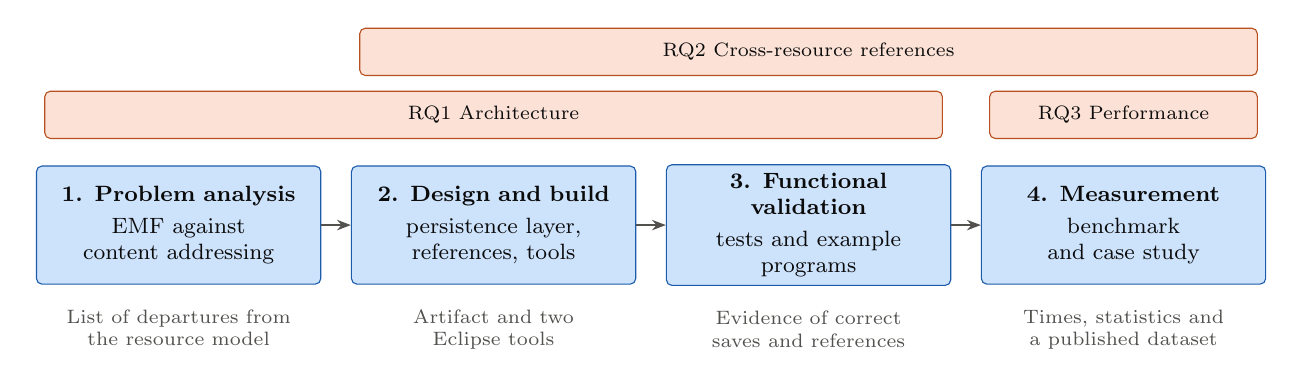
\begin{tikzpicture}[
  font={\footnotesize\hyphenpenalty=10000\exhyphenpenalty=10000},
  >={Stealth[length=5pt]},
  phase/.style={draw=phaseborder, fill=phasefill, rounded corners=2pt, text=ink,
    align=center, text width=34mm, minimum height=15mm, inner sep=3pt, anchor=center},
  outnote/.style={text=inksoft, font={\scriptsize\hyphenpenalty=10000}, align=center,
    text width=36mm, anchor=north},
  question/.style={draw=questionborder, fill=questionfill, rounded corners=2pt, text=ink,
    align=center, minimum height=6mm, inner sep=2pt, font=\scriptsize, anchor=center},
  flow/.style={->, draw=inksoft, line width=0.7pt}
]

\node[phase] (s1) at (0mm,0) {\textbf{1. Problem analysis}\\[2pt] EMF against content addressing};
\node[phase] (s2) at (40mm,0) {\textbf{2. Design and build}\\[2pt] persistence layer, references, tools};
\node[phase] (s3) at (80mm,0) {\textbf{3. Functional validation}\\[2pt] tests and example programs};
\node[phase] (s4) at (120mm,0) {\textbf{4. Measurement}\\[2pt] benchmark and case study};

\draw[flow] (s1) -- (s2);
\draw[flow] (s2) -- (s3);
\draw[flow] (s3) -- (s4);

\node[outnote] at ($(s1.south)+(0,-2mm)$) {List of departures from the resource model};
\node[outnote] at ($(s2.south)+(0,-2mm)$) {Artifact and two Eclipse tools};
\node[outnote] at ($(s3.south)+(0,-2mm)$) {Evidence of correct saves and references};
\node[outnote] at ($(s4.south)+(0,-2mm)$) {Times, statistics and a published dataset};

% A band covers the steps that answer the question.
\node[question, minimum width=114mm] at (40mm,14mm) {RQ1 Architecture};
\node[question, minimum width=34mm] at (120mm,14mm) {RQ3 Performance};
\node[question, minimum width=114mm] at (80mm,22mm) {RQ2 Cross-resource references};
\end{tikzpicture}
\end{document}
